\newcommand{\manydots}[2][9pt]{
\begin{tikzpicture}
\foreach \x in {1,...,#2} 
\fill (\x*#1,0) circle (0.55pt);
\end{tikzpicture}
}

\renewcommand{\therefore}{
\ensuremath{
\mathrel{
\begin{tikzpicture}[scale=0.18]
\fill (0,0) circle (5pt);
\fill (1,0) circle (5pt);
\fill (60:1) circle (5pt);
\end{tikzpicture}} }}

\renewcommand{\because}{
\ensuremath{
\mathrel{
\begin{tikzpicture}[scale=-0.18]
\fill (0,0) circle (5pt);
\fill (1,0) circle (5pt);
\fill (60:1) circle (5pt);
\end{tikzpicture}} }}

\newcommand{\equals}{
\ensuremath{
\mathrel{
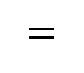
\begin{tikzpicture}[baseline=-1.0ex]
\draw[line width=1.0pt] (0,1.5pt) -- (9pt,1.5pt);
\draw[line width=1.0pt] (0,-1.5pt) -- (9pt,-1.5pt);
\end{tikzpicture}}}
}

\newcommand{\notequals}{
\ensuremath{
\mathrel{
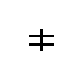
\begin{tikzpicture}[baseline=-0.5ex]
\draw[line width=1.0pt] (0,1.5pt) -- (9pt,1.5pt);
\draw[line width=1.0pt] (0,-1.5pt) -- (9pt,-1.5pt);
\draw[line width=1.0pt] (4.5pt,-4pt) -- (4.5pt,4pt);
\end{tikzpicture}}}
}

\newcommand{\greater}{
\ensuremath{
\mathrel{

\begin{tikzpicture}
\draw[line width=1.0pt] (9pt,2.5pt) -- (0,2.5pt) -- (0,-2.5pt) -- (9pt,-2.5pt);
\end{tikzpicture}}}
}
\newcommand{\less}{
\ensuremath{
\mathrel{
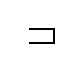
\begin{tikzpicture}[scale=-1]
\draw[line width=1.0pt] (9pt,2.5pt) -- (0,2.5pt) -- (0,-2.5pt) -- (9pt,-2.5pt);
\end{tikzpicture}}}
}
\newcommand{\notgreater}{
\ensuremath{
\mathrel{

\begin{tikzpicture}
\draw[line width=1.0pt] (9pt,2.5pt) -- (0,2.5pt) -- (0,-2.5pt) -- (9pt,-2.5pt);
\draw[line width=1.0pt] (4.5pt,-5pt) -- (4.5pt,5pt);
\end{tikzpicture}}}
}
\newcommand{\notless}{
\ensuremath{
\mathrel{

\begin{tikzpicture}[scale=-1]
\draw[line width=1.0pt] (9pt,2.5pt) -- (0,2.5pt) -- (0,-2.5pt) -- (9pt,-2.5pt);
\draw[line width=1.0pt] (4.5pt,-5pt) -- (4.5pt,5pt);
\end{tikzpicture}}}
}
\newcommand{\plus}{
\ensuremath{
\mathbin{
\begin{tikzpicture}
\draw[line width=1.0pt] (0pt,-4pt) -- (0pt,4pt);
\draw[line width=1.0pt] (-4pt,0pt) -- (4pt,0pt);
\end{tikzpicture}}}
}
\newcommand{\minus}{
\ensuremath{
\mathbin{
\begin{tikzpicture}
\draw[line width=1.0pt] (-4pt,0pt) -- (4pt,0pt);
\end{tikzpicture}}}
}
\newcommand{\cross}{
\ensuremath{
\mathbin{

\begin{tikzpicture}[rotate=45]
\draw[line width=1.0pt] (0pt,-4pt) -- (0pt,4pt);
\draw[line width=1.0pt] (-4pt,0pt) -- (4pt,0pt);
\end{tikzpicture}}}
}
\newcommand{\isto}{
\ensuremath{
\mathrel{
\begin{tikzpicture}
\fill (0,1.5pt) circle (1pt);
\fill (0,-1.5pt) circle (1pt);
\end{tikzpicture}}}
}
\newcommand{\as}{
\ensuremath{
\mathrel{

\begin{tikzpicture}
\fill (-1.5pt,1.5pt) circle (1pt);
\fill (-1.5pt,-1.5pt) circle (1pt);
\fill (1.5pt,1.5pt) circle (1pt);
\fill (1.5pt,-1.5pt) circle (1pt);
\end{tikzpicture}}}
}

\newcommand{\plel}{
\ensuremath{
\mathrel{

\begin{tikzpicture}
\draw[line width=1pt] (-1.2pt,-4.0pt) -- (-1.2pt,4.0pt);
\draw[line width=1pt] (1.2pt,-4.0pt) -- (1.2pt,4.0pt);
\end{tikzpicture}}}
}
\newcommand{\perpendicular}{
\ensuremath{
\mathrel{
\begin{tikzpicture}
\draw[line width=1pt] (0pt,6.0pt) -- (0pt,0pt);
\draw[line width=1pt] (-4.0pt,0pt) -- (4.0pt,0pt);
\end{tikzpicture}}}
}

\newcommand{\acuteangle}{
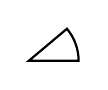
\begin{tikzpicture}[thick]
\draw (0,0) -- (18pt,0) arc (0:40:18pt) -- cycle;
\end{tikzpicture}
}
\newcommand{\rightangle}{

\begin{tikzpicture}[thick]
\draw (0,0) -- (18pt,0) arc (0:90:18pt) -- cycle;
\end{tikzpicture}
}
\newcommand{\rightangles}{
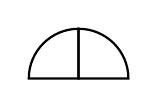
\begin{tikzpicture}[thick]
\draw (0,0) -- (18pt,0) arc (0:90:18pt) -- cycle;
\draw (0,0) -- (0,18pt) arc (90:180:18pt) -- cycle;
\end{tikzpicture}
}
\newcommand{\vertex}{

\begin{tikzpicture}[scale=0.35,ultra thick,rotate=-93]
\draw (0,0) -- (1,0) -- (0,0) -- (40:1);
\end{tikzpicture}
}
\newcommand{\trivertex}{
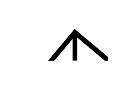
\begin{tikzpicture}[scale=0.6,ultra thick,rotate=-130]
\clip[rotate=130] (-1,-0.6) rectangle (0.7,0.1);
\draw (90:1) -- (0,0) -- (1,0);
\draw (1,0) -- (0,0) -- (90:1);
\draw (0,0) -- (40:1);
\end{tikzpicture}
}

